\documentclass[10pt,twocolumn,letterpaper]{article}

\usepackage{cvpr}
\usepackage{times}
\usepackage{epsfig}
\usepackage{graphicx}
\usepackage{amsmath}
\usepackage{amssymb}

% Include other packages here, before hyperref.

% If you comment hyperref and then uncomment it, you should delete
% egpaper.aux before re-running latex.  (Or just hit 'q' on the first latex
% run, let it finish, and you should be clear).
%\usepackage[pagebackref=true,breaklinks=true,letterpaper=true,colorlinks,bookmarks=false]{hyperref}

\cvprfinalcopy % *** Uncomment this line for the final submission

\def\cvprPaperID{1} % *** Enter the CVPR Paper ID here
\def\httilde{\mbox{\tt\raisebox{-.5ex}{\symbol{126}}}}

% Pages are numbered in submission mode, and unnumbered in camera-ready
\ifcvprfinal\pagestyle{empty}\fi
\begin{document}

%%%%%%%%% TITLE
\title{ Program 1: Feature Detection, Extraction/Description, and Matching}

\author{Brian Fehrman\\
SDSM\&T\\
501 E. Saint Joseph Street\\
{\tt\small bcfehrman@gmai1.com}
\thispagestyle{empty}
}

\maketitle
%%%%%%%%% ABSTRACT
\begin{abstract}
In this work I explored feature detection, extraction/description, and matching. The method implemented was a version of the Harris-Laplace method which offers scale, rotation, and illumination invariance when properly implemented. In addition to this, adaptive non-maximum suppression was also implemented and found to have better results than just picking the features with the largest response. A special pruning algorithm has also been implemented during the matching stage which will not allow for multiple matches to the same point and instead will pick the best pair of matches. This pruning along with using the ratio test (instead of just the SSD) was found to get rid of a large amount of the false matches that were present before implementing these techniques. All bench mark images were tested using the same tuning variable values such as the smoothing/derivation scales and the thresholds. Lastly, the algorithm was extended to work on live video feed and is able to track features between successive frames quite well.

\end{abstract}

%%%%%%%%% BODY TEXT


\section{Introduction}
The purpose of this project was to implement multiple algorithms with the ultimate goal of matching features between two slightly different images. This involved feature detection, feature extraction and description, and feature matching algorithms that needed to be implemented. Each of these algorithms will be detailed in the following sections.

%----------------------------1---------------------------------------------
\section{Feature Detection}

For the feature detection stage I used the Harris corner detector as shown in the Szeliski book and as covered in class. This algorithm simply computes the image gradients in both directions using a gaussian derivative kernel. For my algorithm, I chose a standard deviation of 1.5 and a kernel size of 5. The resulting x derivative image, $I_x$, was point-wise squared. This was done for the y derivative image, $I_y$, as well. The x and y derivative images were also point-wise multiplied so that three new images resulted, $I_x^2, I_y^2, I_xI_y$. These three images were then smoothed using a standard deviation of 1.4 and used to determine the corner strength function for each point in the original image. This strength was thresholded with a value of 0.01 with all responses lower than this being discarded. All feature points have their response strength placed in to a matrix in which the position is the same as the point's position in the original image. All spots in the matrix that weren't filled are set to be 0.


\section{Adaptive Non-Maximum Suppression}
After finding feature points and creating the matrix containing those threshold values, adaptive non-maximum suppression is then applied in which it is required that all feature points be a local maximum withing a 25 points radius and be greater than 10 percent in response value than the points in that radius. Any point not meeting the preceding requirements are zeroed out. All points that are kept are placed in to a vector. This proved to give a much better distribution of feature points than just choosing the points the highest responses.

\section{Feature Extraction / Description}
The program then runs through the vector of feature points and performs a Laplacian of Gaussian for each point at multiple scales and determines which scale provides the largest response. This is chosen as the characteristic scale of that feature. A feature region around the point is then extracted at the dominant scale. The dominant orientation of the feature is determined by running x and y derivative kernels over the extracted feature region and averaging the values for each derivative. These averaged derivative values for the x and y directions and the atan2 function are used to determine the dominant angle orientation of the feature. Once the dominant angle was determined, a larger region around the feature was extracted and a rotated patch the size of the feature was extracted from that region by using the simple rotation matrix equation and inserting negative of the dominant orientation angle into the trig functions. Once the feature had been oriented its intensity values were then normalized. 

\section{Feature Matching}
Matching was done using both the SSD and the SSD with ratio testing, as described in the program requirements. An additional pruning algorithm was implemented such that the program keeps track of each point in the second image that has been matched. Any new potential matches to a previously matched point are compared and the better of the two matches is kept. There is more to it but I'm getting really tired at this point =). This also helped enormously in eliminating false matches and cleaning up the output of the program.

\section{Results}
The program proved to work quite well. It fails biggest on graffiti, as would be expected since it doesn't really contain an affine inavariant feature descriptor. It does ok on the first two images of graffiti but very poorly has the successive images have more and more out of plane rotation. I am not entirely sure that I have the Harris-Laplace implemented correctly but I believe that it is close. What I found most impressive was that I didn't need to change any parameters between image sets and that the same set of values worked pretty well for all of the image sets. You can draw your own conclusions though. I have also extended this to work on webcam feed and it does quite well at tracking features between frames. I have a few videos. One set is full speed and has both a matching video and a video which just shows the features. The second video sets have a delay between frames to get a better idea of the invariance of the algorithm to larger changes between the frames. They also seem to do ok.

\begin{figure*}[ht!]
\centering
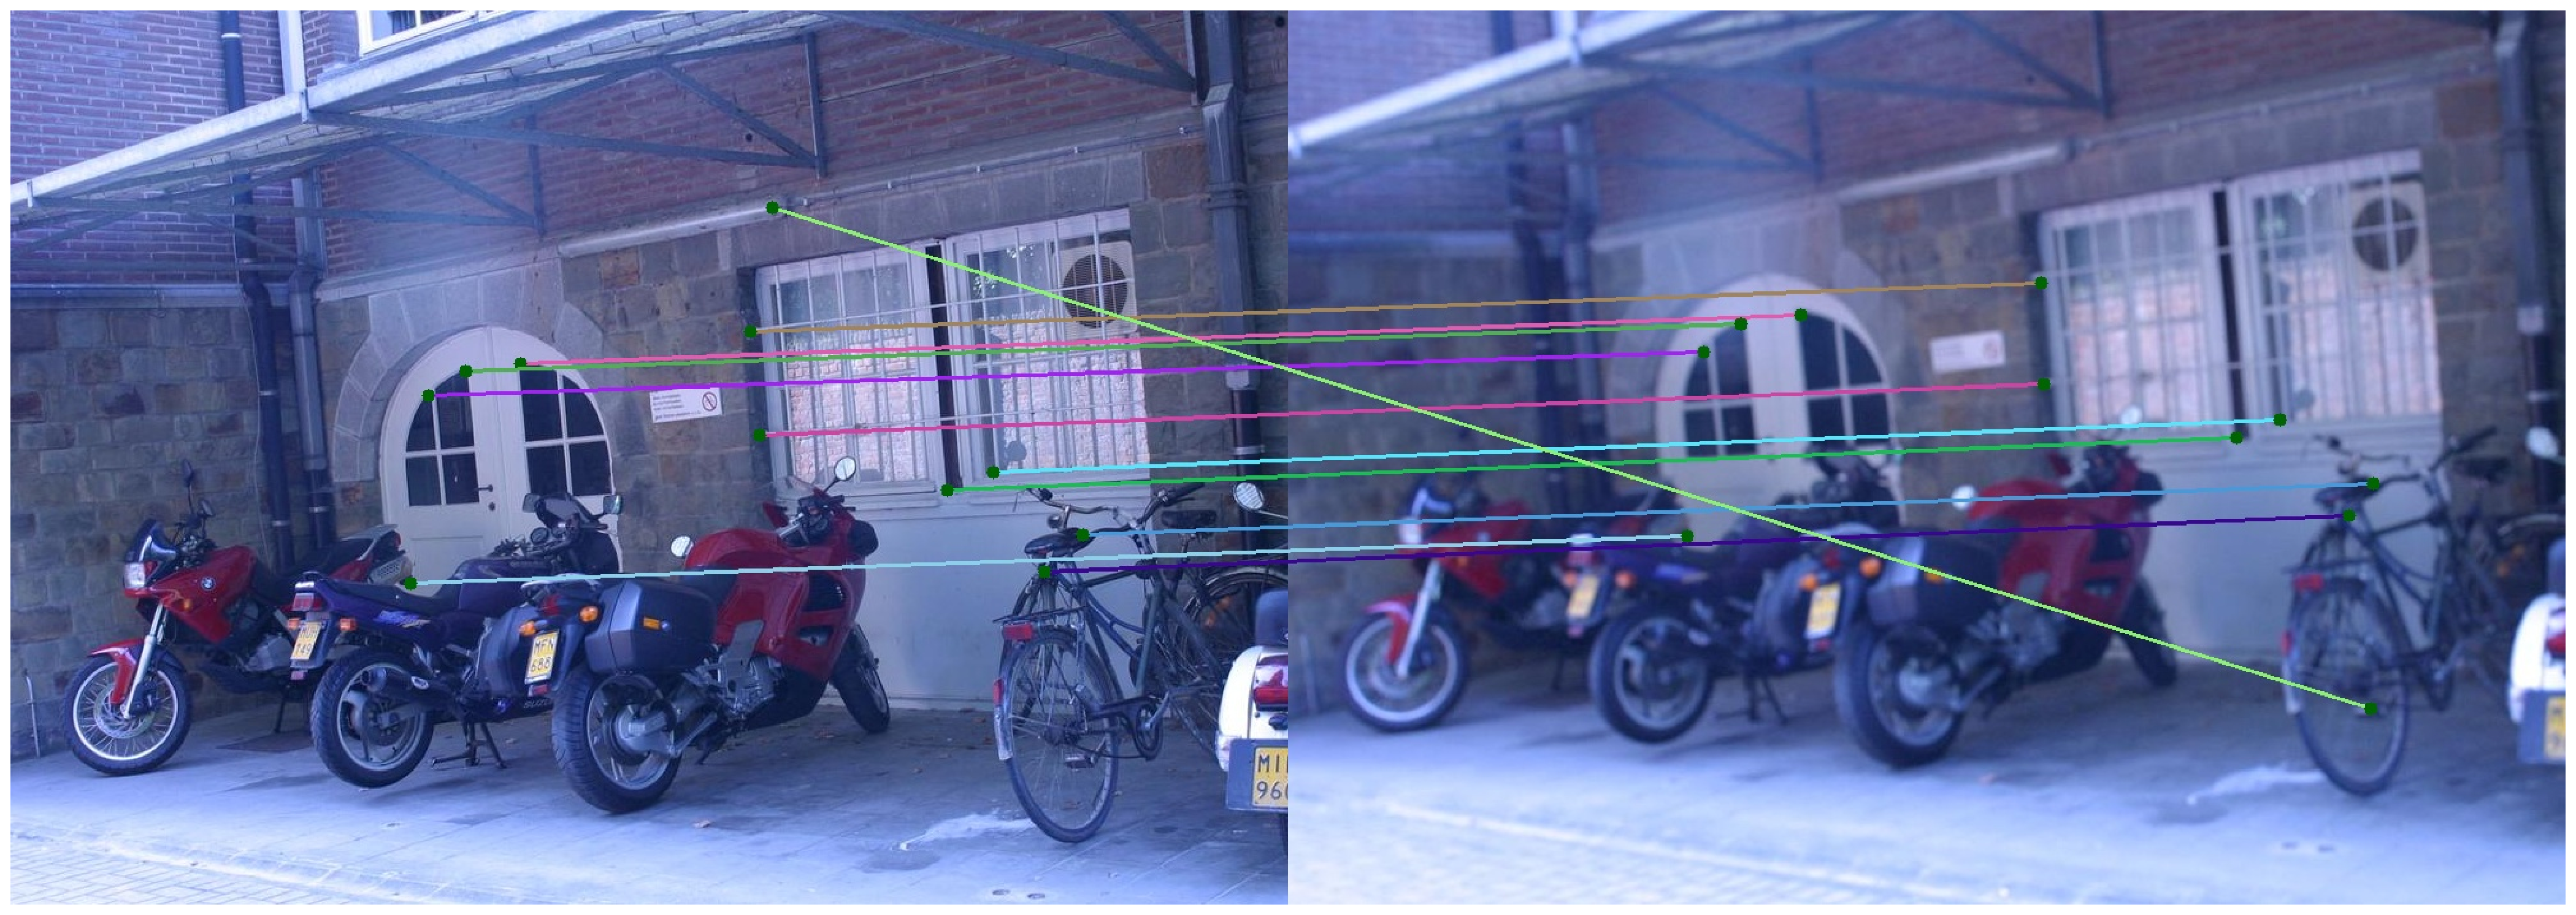
\includegraphics[width=1\textwidth]{img/bikes1_4_ratio.eps}
\caption{Bikes images 1 and 4}
\label{fig:bikes}
\end{figure*}

\begin{figure*}[ht!]
\centering
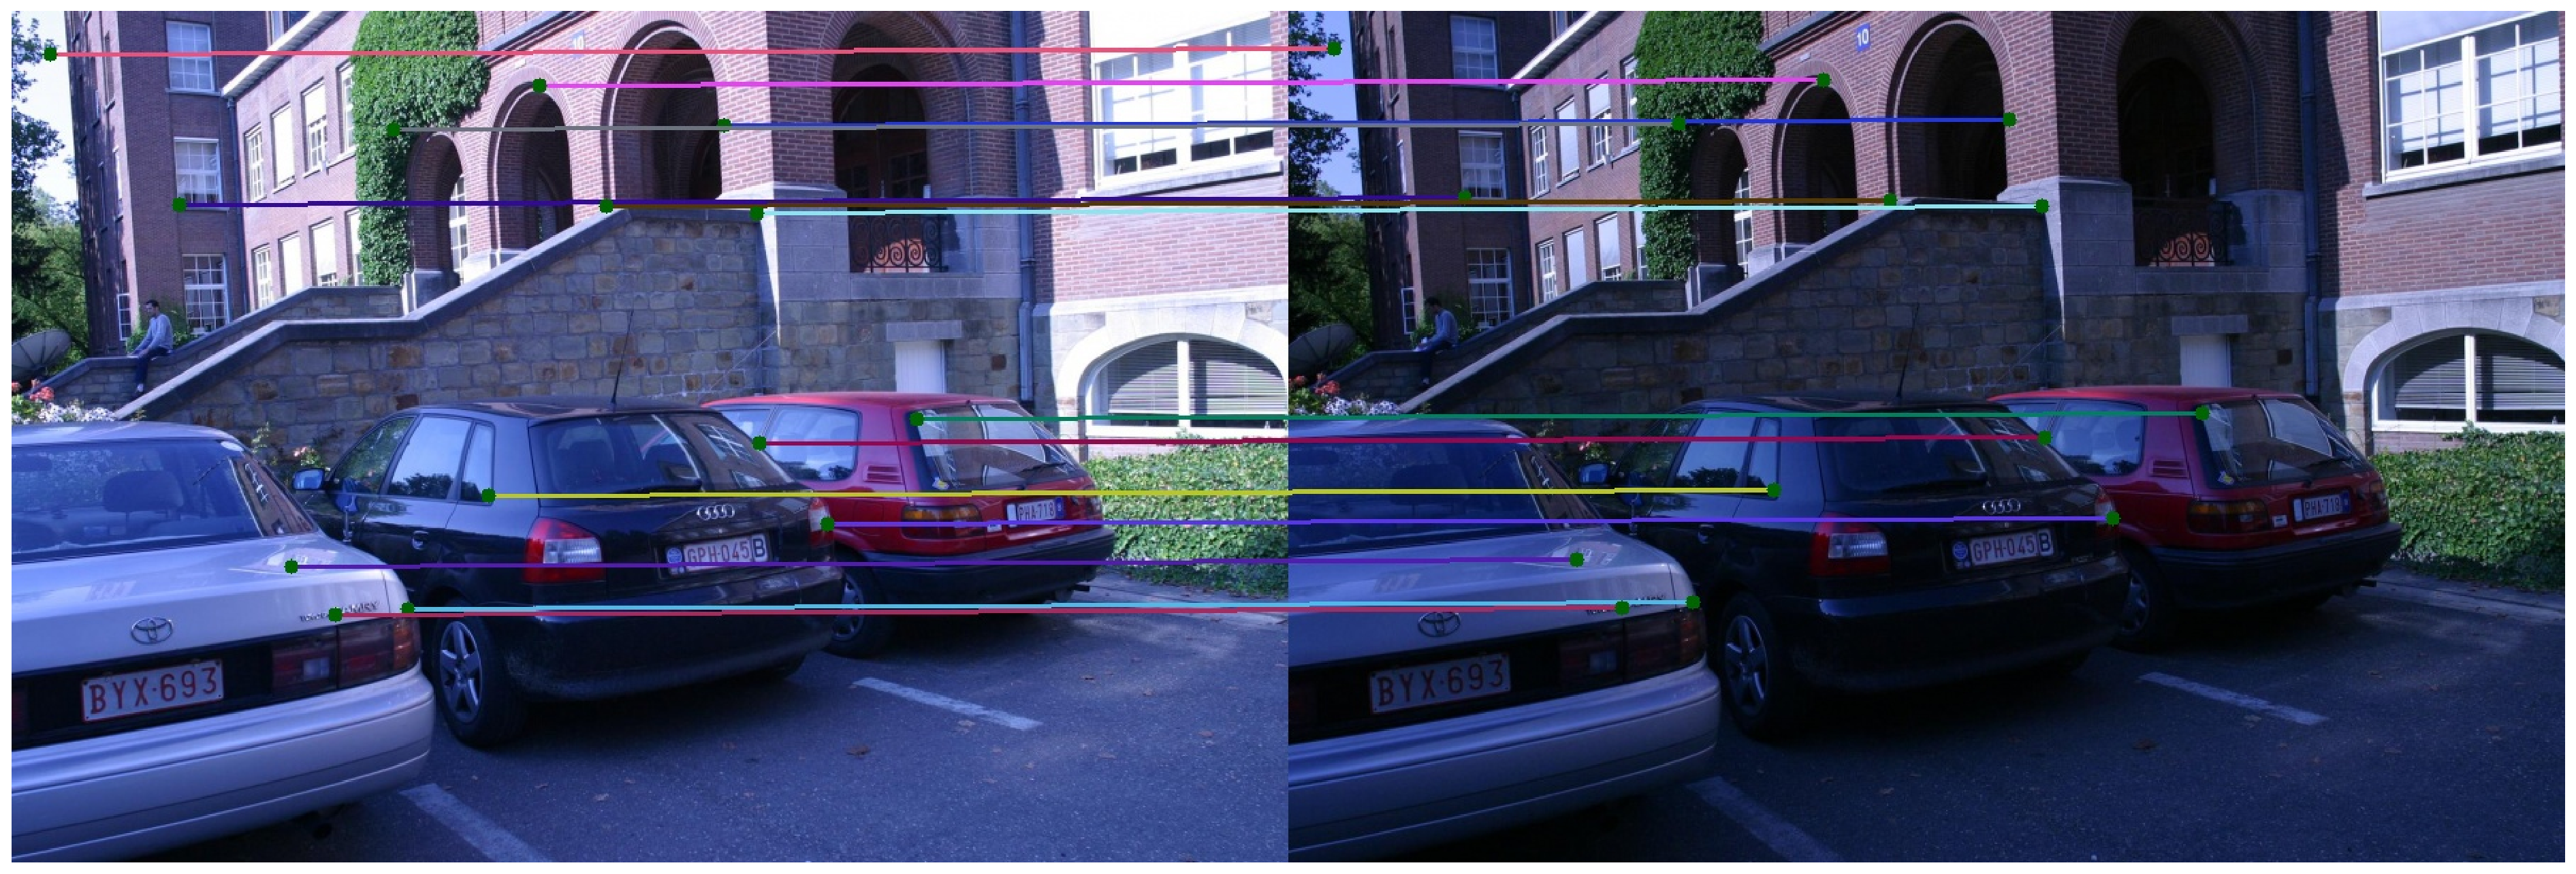
\includegraphics[width=1\textwidth]{img/leuven1_3_ratio.eps}
\caption{Leuven images 1 and 3}
\label{fig:leuven}
\end{figure*}

\begin{figure*}[ht!]
\centering
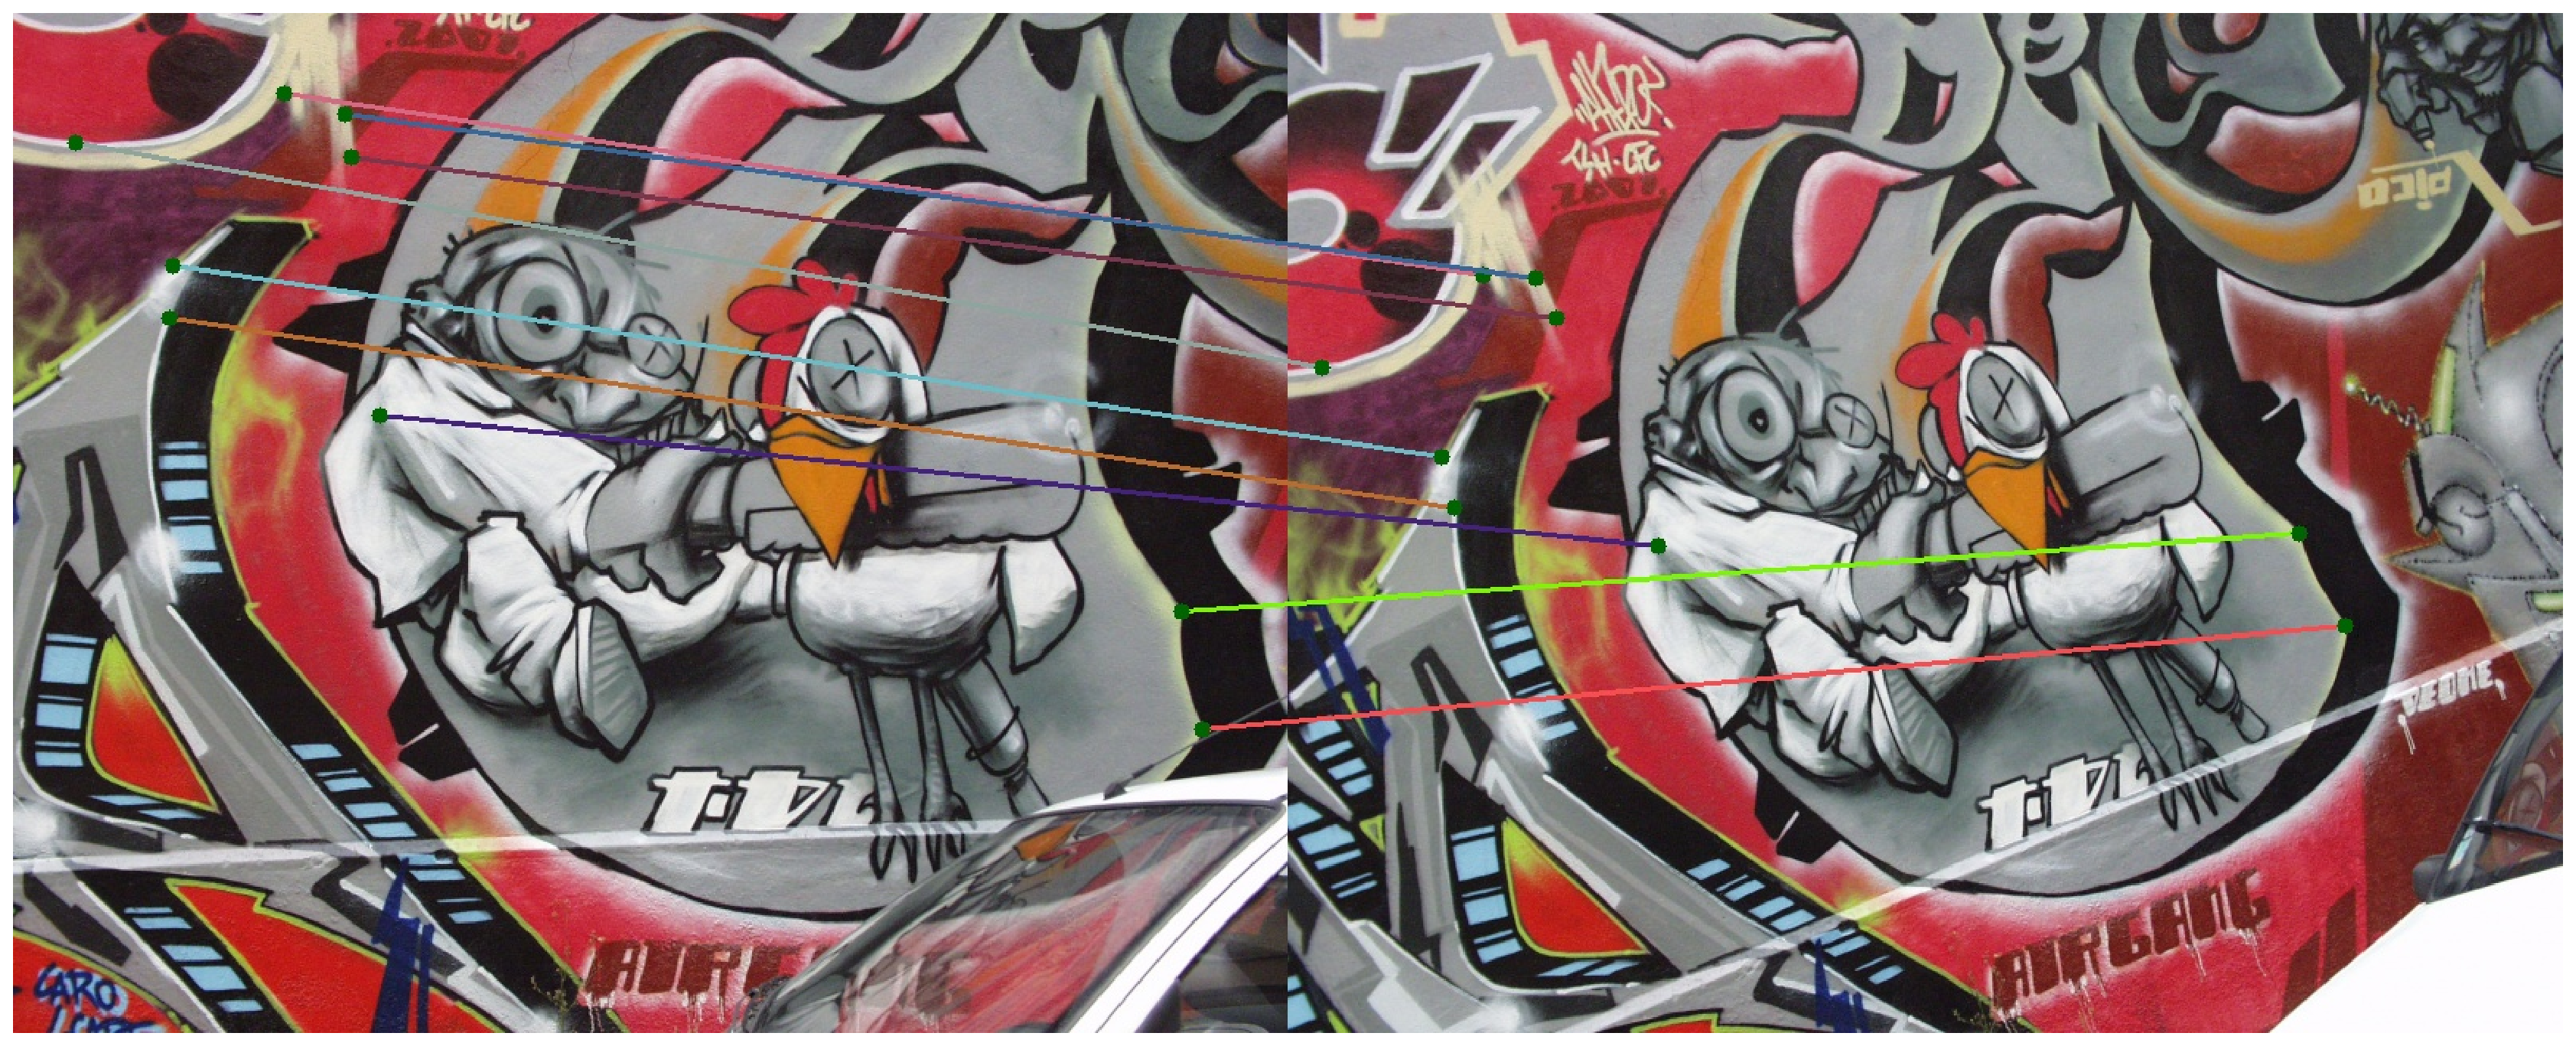
\includegraphics[width=1\textwidth]{img/graf1_2_ratio.eps}
\caption{Graf images 1 and 2}
\label{fig:graf}
\end{figure*}

\begin{figure*}[ht!]
\centering
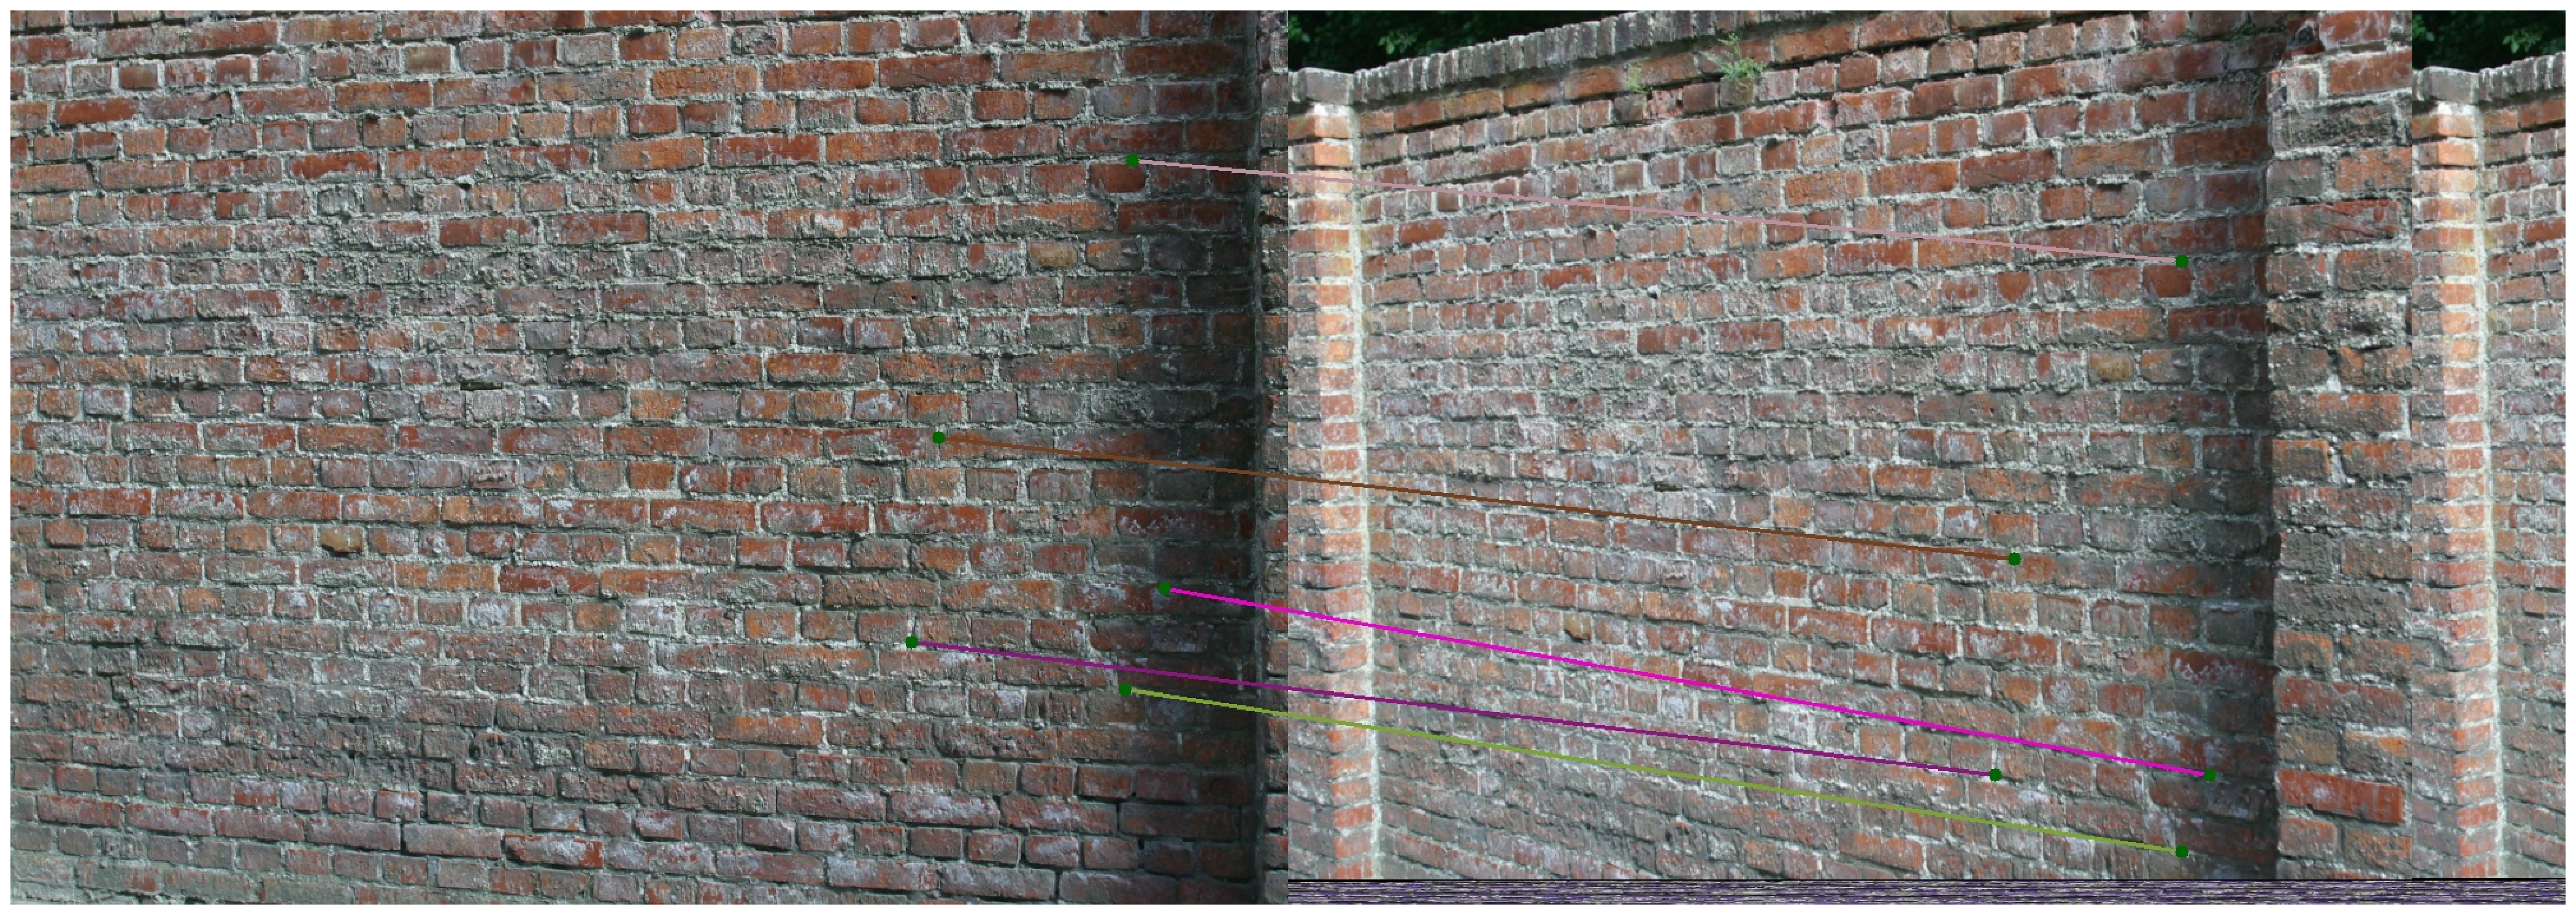
\includegraphics[width=1\textwidth]{img/wall1_3_ratio.eps}
\caption{Wall images 1 and 3}
\label{fig:wall}
\end{figure*}

\begin{figure*}[ht!]
\centering
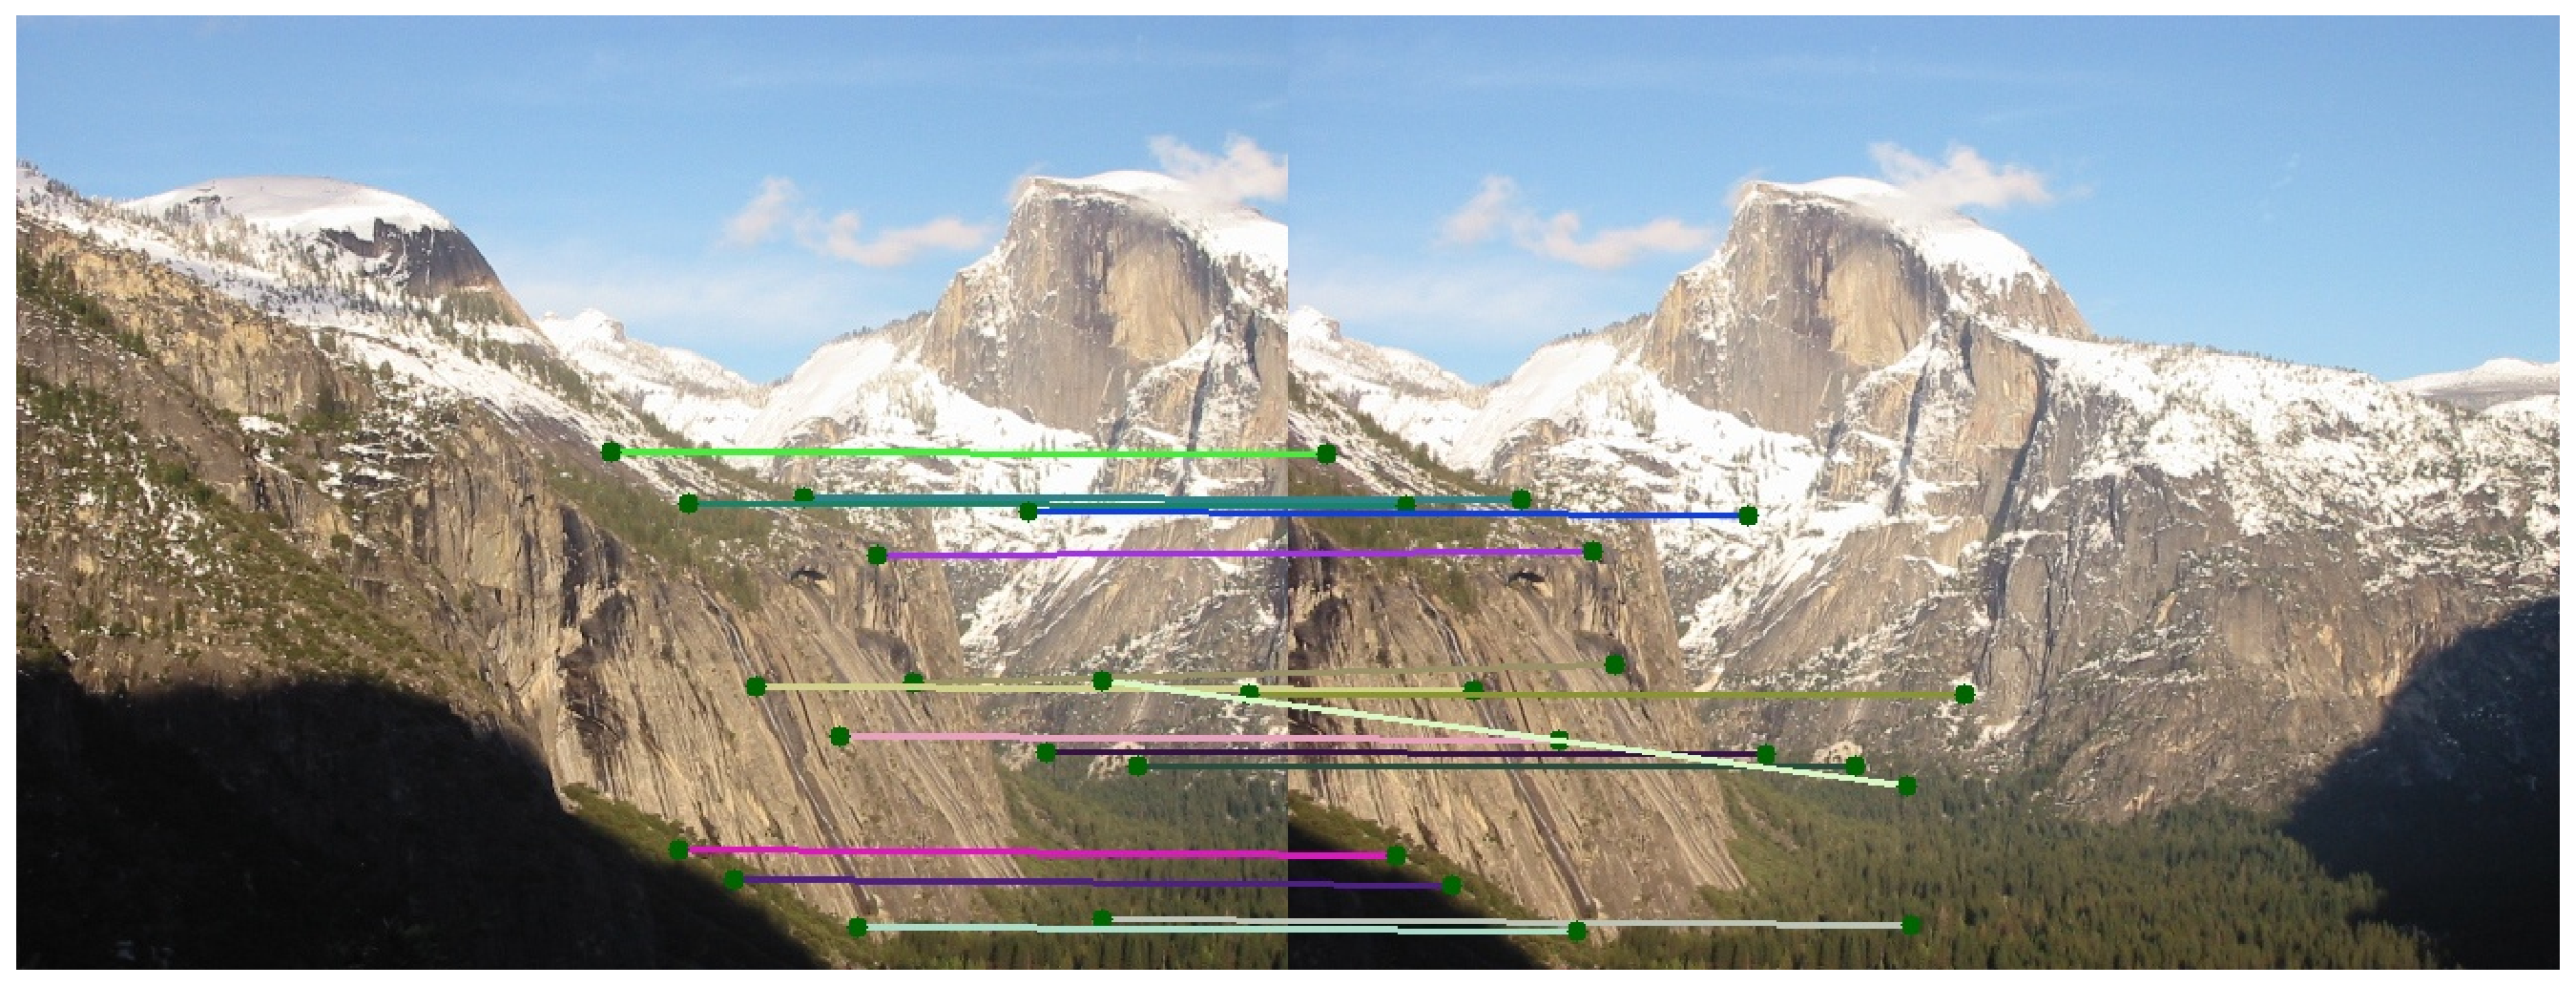
\includegraphics[width=1\textwidth]{img/Yosemite1_2_ratio.eps}
\caption{Yosemite images 1 and 2}
\label{fig:yosemite}
\end{figure*}

\begin{figure*}[ht!]
\centering
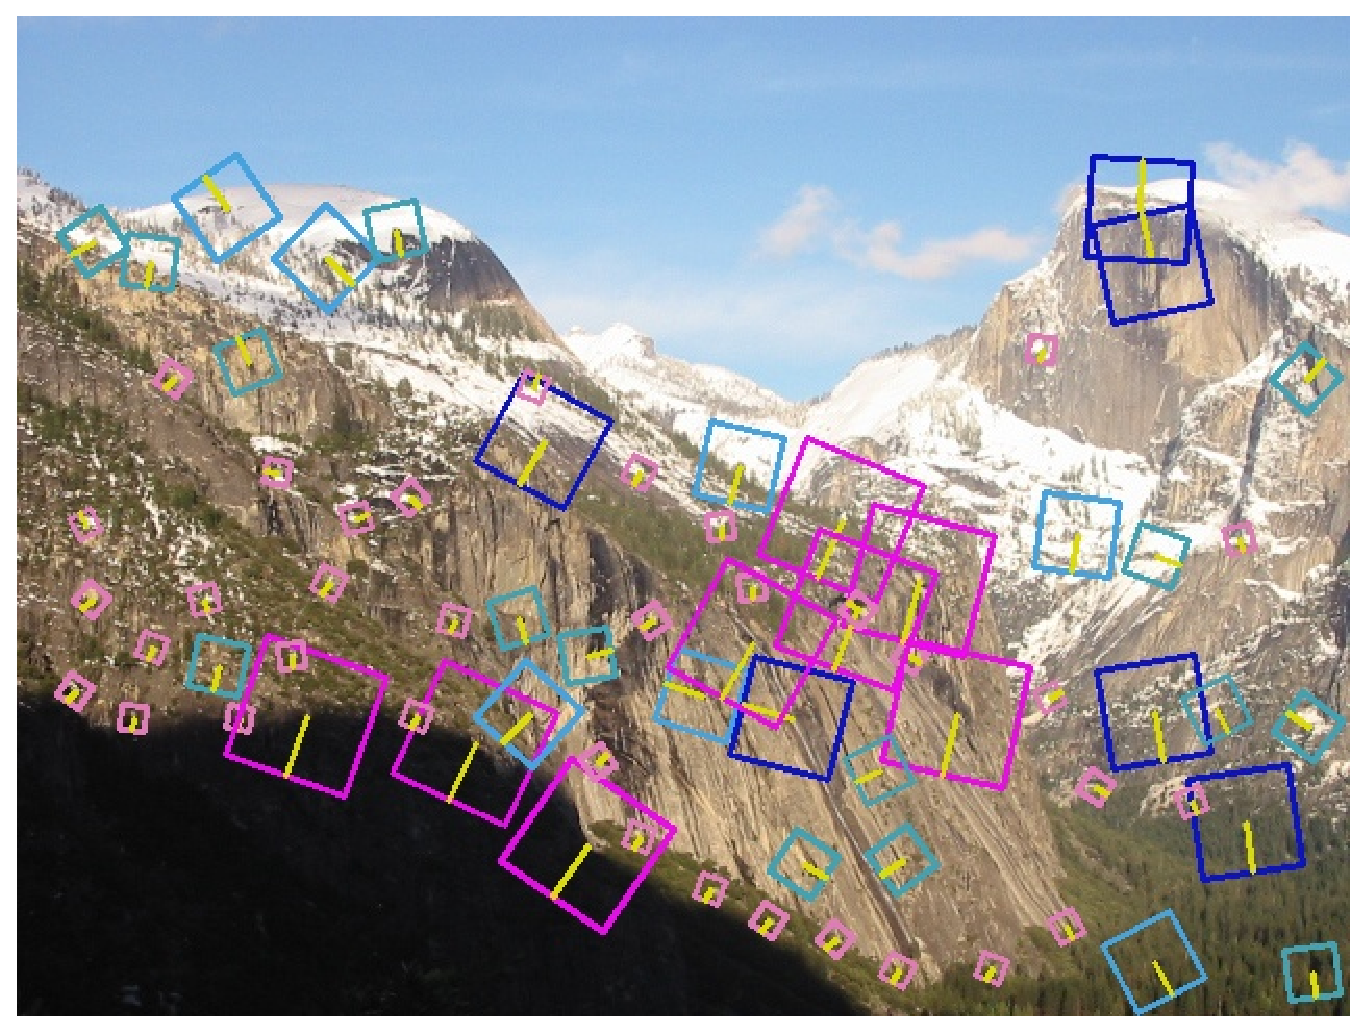
\includegraphics[width=1\textwidth]{img/Yosemite1_features.eps}
\caption{Yosemite features}
\label{fig:yosemite_feat}
\end{figure*}

{\small
\bibliographystyle{ieee}
\bibliography{egbib}
}

\end{document}
